% Preambule
\documentclass[pdftex,french, english]{article}	% the pdftex is essential

% Packages
% ---
\usepackage[utf8]{inputenc}
\usepackage[T1]{fontenc}
\usepackage[dvips]{graphicx}            % to include images
\usepackage{pslatex}	    % to use PostScript fonts
\usepackage{enumitem}
\usepackage{amsfonts}
\usepackage{babel}
\usepackage{algorithm}
\usepackage[noend]{algpseudocode}
\usepackage[paperwidth=17cm, paperheight=22.5cm, bottom=2.5cm, right=2.5cm]{geometry}
\usepackage{csquotes}
\usepackage{multirow}
\usepackage{caption}
\usepackage{hyperref}
\usepackage{subcaption}
\usepackage{tikz}


% where to find images:
\graphicspath{{../images/}}

\setcounter{secnumdepth}{4}
\setcounter{tocdepth}{3}
\makeatletter
\newcounter {subsubsubsection}[subsubsection]
\renewcommand\thesubsubsubsection{\thesubsubsection .\@alph\c@subsubsubsection}
\newcommand\subsubsubsection{\@startsection{subsubsubsection}{4}{\z@}%
                                     {-3.25ex\@plus -1ex \@minus -.2ex}%
                                     {1.5ex \@plus .2ex}%
                                     {\normalfont\normalsize\bfseries}}
\newcommand*\l@subsubsubsection{\@dottedtocline{3}{10.0em}{4.1em}}
\newcommand*{\subsubsubsectionmark}[1]{}
\makeatother

\begin{document}
\selectlanguage{english}

\title{INITIATION A LA RECHERCHE}

\begin{titlepage}
\begin{center}

\textsc{\Large Initiation à la recherche}\\[4em]

\begin{figure}[h]
\begin{center}
\includegraphics[width=5cm,height=6cm,keepaspectratio]{lorraine.png}
\end{center}
\end{figure}

\vspace{4em}
\textsc{\Large \textbf{Planification d'actions \\ dans un monde continu}}\\[10em]
\textsc{\textit{Léopold BELLEC, Pierre-Marie JUNGES}}\\[1em]
\vspace{1em}
\textsc{Encadrants : \textit{Olivier BUFFET, Vincent THOMAS}}\\[1em]


\end{center}

\vspace*{\fill}
\textsc{Master 1 Informatique \hspace*{\fill} 2017}

\end{titlepage}

\newpage
\pagenumbering{arabic}

\selectlanguage{french}
\tableofcontents


\newpage
\selectlanguage{english}
\section{Introduction au problème}
	\subsection{Problématique}
	Une des problématiques importantes en intelligence artificielle est la planification automatique d’actions, que ce soit pour la robotique, pour les jeux (échecs, go, ...), pour la gestion de sources d’énergie, ou pour la protection d’espèces menacées. La plupart des algorithmes développés n’abordent que des situations dans lesquelles le nombre d’états (le nombre de situations) possibles est fini et relativement petit, tout comme le nombre d’actions disponibles. Ces limitations viennent de ce que ces algorithmes raisonnent sur l’arbre des évolutions possible du “système” à contrôler, arbre dont la taille subit une explosion combinatoire avec les nombres d’états et d’actions (et qui n’a plus de sens quand les facteurs de branchement sont infinis).
	\subsection{En quoi ce sujet est-il intéressant ?}

	La principale raison est que les algorithmes que nous allons étudier permettent de résoudre des problèmes proches de l'environnement réel.

	En effet, ces algorithmes peuvent résoudre des problèmes auxquels nous sommes régulièrement confrontés, par exemple, lorsque l'on suit quelqu'un en marchant, inconsciemment, nous faisons en sorte que notre vitesse ne soit pas plus rapide (resp. lente) que la personne que nous suivons, nous devons donc accélérer ou réduire notre vitesse.

	Et bien, c'est exactement le genre de problème que ces algorithmes peuvent résoudre.

	De plus, une variante de cet algorithme permettra de gérer des cas où un événement tiers perturbe les résultats, si nous faisons encore le parallèle avec le monde réel, cet événement peut être un coup de vent ou bien une glissade.

	C'est pourquoi, nous avons souhaité prendre ce sujet et pousser un peu plus nos connaissances sur les algorithmes de décisions.
	
	\subsection{Notre approche}
	Étant donné le nombre imposant d'états ou d'actions possibles, nous avons donc tout simplement essayé, à chaque étape, de réduire ce nombre de choix possible jusqu'à obtenir un espace plus restreint et donc plus facilement exploitable \cite{couetoux01}.

	C'est donc la solution que nous avons choisie pour répondre à cette problématique. 

	Afin de pouvoir mettre en place nos algorithmes, nous avions deux choix d'implémentations, utiliser le langage C ou bien le langage Java. 
	Notre choix s'est finalement porté sur le langage Java, car nous sommes plus habitués à ce dernier et nous trouvons la gestion de mémoire également plus simple.

\section{Le B.A.-BA de l'algorithme MCTS}

	Dans cette partie nous allons introduire les notions importantes relatives à l'algorithme \textbf{M}onte \textbf{C}arlo \textbf{T}ree \textbf{S}earch \cite{coulom01}
	appliqué à un problème discret, c'est-à-dire un problème où le nombre d'états ou actions est fini.

	\subsection{Les bases du Monte Carlo Tree Search}
	\subsubsection{Définition}
	Monte Carlo Tree Search ou bien MCTS est un algorithme de recherche, qui, à partir d'un nœud initial $n_{i}$ indique la meilleure action $a_i$ à utiliser afin d'atteindre un nœud intermédiaire $n_{int}$ proche du nœud terminal recherché $n_{t}$. 

	L'application de méthodes de Monte Carlo fait appel à de nombreuses simulations, cela veut donc dire que lors du déroulement de l'algorithme, un certain nombre d'actions seront joués de manière aléatoire.
	\subsubsection{Déroulement de l'algorithme}
	L'algorithme est exécuté tant que le temps limite $t$ n'est pas écoulé, et se décompose en 4 étapes :
	\begin{figure}[h]
		\centering
		\includegraphics[width=\textwidth]{etapes.png}
		\caption{ Étapes de MCTS}
		 \label{fig:mcts}
	\end{figure}

\textit{Notation : Le nœud correspond à un état du jeu et (12/21) signifie 12 victoires sur 21 simulations.} 
	\begin{enumerate}
		\item \textbf{Sélection}

		À cette étape, l'algorithme va sélectionner parmi ses nœuds suivants le nœud avec la plus grande valeur selon la formule de sélection utilisée dans la partie \ref{selection}. 

		Dans la figure~\ref{fig:mcts}, on s'aperçoit que l'algorithme sélectionne à tour de rôle le nœud $(7/10)$, puis le nœud $(5/6)$ et enfin le nœud $(3/3)$ et s'arrête car ce nœud n'est pas développé.
		\item \textbf{Expansion}

		Une fois le meilleur nœud sélectionné, cette étape va lui rajouter un ou plusieurs nœud(s) enfant, accessible en faisant 1 seule action à partir du nœud courant. 

		Dans la figure~\ref{fig:mcts}, l'algorithme rajoute au nœud courant $(3/3)$ le nœud enfant $(0/0)$.
		\item \textbf{Simulation}

		Maintenant qu'un nouveau nœud a été ajouté, l'algorithme va jouer aléatoirement jusqu'à atteindre un nœud terminal.
		C'est dans cette partie qu'on utilise le principe Monte Carlo, c'est-à-dire l'utilisation de l'aléatoire.
		\item \textbf{Mise à jour} 

		L'algorithme a atteint un nœud terminal, il faut donc récupérer sa récompense (par exemple +1 si c'est un nœud gagnant 0 sinon). Puis faire remonter cette récompense jusqu'au nœud racine et mettre à jour les statistiques de chacun des nœuds parcourus. 

		Dans la figure~\ref{fig:mcts} ci-dessus le nœud terminal était donc perdant car $(0/1)$, donc on va augmenter uniquement le nombre de simulation de chacun de ces nœuds, d'où la transformation du nœud $(3/3)$ en $(3/4)$ par exemple.
	\end{enumerate}
	\subsubsection{Pseudo-code}
	\begin{algorithm}
	\caption{MCTS générique}
	  \label{alg:mcts}
	\begin{algorithmic}[1]
	\Function{MCTS}{État $s$}
	\State création d'un nœud $n$ à partir de $s$
		\While{$temps < tempsLimite $}\Comment{tant qu'il reste du temps}
			\State $n \gets selection(n)$ \Comment{L'étape d'expansion est incluse dans cet appel}
			\State $n \gets simulation(n)$
			\State $n \gets miseAjour(n)$
		\EndWhile
	\State \textbf{return} $meilleurEnfant(n)$
	\EndFunction
	\end{algorithmic}
	\end{algorithm}
    
    
	\subsection{Formule de sélection utilisée} \label{selection}
	Précédemment, nous avions parlé lors de l'étape de sélection, de formule de sélection. 
	En effet, afin de choisir le meilleur nœud possible des formules ont été mises en place.


	Et, c'est dans cette partie que nous allons en expliquer une (la principale utilisée), puis de nouvelles seront introduites
	dans la partie \ref{continu}. \\

	\textit{Notation : Soit $n$ un nœud, $N$ son nœud parent, et C une constante d'exploration.} \\

	Upper Confidence Bounds (\textbf{UCB}) :
		\[ \frac{recompenses(n)}{simulations(n)} + C \times \sqrt{\frac{simulations(N)}{simulations(n)}} \] 

		On se rend compte ici que si notre constante d'exploration \textit{C} est égale à $0$ alors, l'algorithme va choisir le nœud $n$ avec le meilleur rapport $\frac{recompenses(n)}{simulations(n)}$ possible. 

		Donc si l'on souhaite permettre l'exploration de l'arbre, il faut que la constante $C$ soit différente de $0$ sinon on voit bien qu'à l'état initial l'algorithme sélectionne un nœud $n$, alors ce dernier aura nécessaire le meilleur rapport $\frac{recompenses(n)}{simulations(n)}$ vu qu'il est le seul à avoir été développé et,  il sera tout au long de l'algorithme choisit. 


		\underline{\textbf{Lexique}} : On utilise le terme UCT (\textit{Upper Confidence Bound for Trees}) pour désigner l'algorithme MCTS utilisant une formule de sélection de type UCB.





	\subsection{Stratégies de sélection terminale} \label{selectionFinale}
	Les formules explicitées ci-dessus ont pour rôle de choisir le meilleur enfant lorsque l'algorithme se trouve à l'étape de sélection. 

	Dans cette partie, l'algorithme est terminé et l'arbre a été développé. Nous ne pouvons donc plus réutiliser les formules précédentes car la constante d'exploration \textit{C} n'a plus de sens ici. 

Il faut donc trouver d'autres moyens pour choisir le meilleur nœud enfant. 
Cette étape correspond à l'appel \textit{meilleurEnfant(n)} dans l'algorithme~\ref{alg:mcts}. 
Or, nous savons qu'un nœud $n$ possède un nombre de simulation et, de récompense.
	À partir de ces deux informations nous avons utilisé 3 stratégies de sélection :
	\begin{enumerate}
		\item Robuste : 
		
		On choisit le nœud avec le plus grand nombre de simulation.
		\item Maxi :  
		
		On choisit le nœud qui possède la valeur de récompense la plus élevée.
		\item Maxi-Robuste :
		
		On choisit le nœud ayant le meilleur rapport $\frac{recompense}{simulation}$.
	\end{enumerate}
    
    
    
    
    
	\subsection{Application sur un exemple} \label{P4}
	Maintenant que nous avons vu comment l'algorithme fonctionnait de manière générale, mettons le en pratique sur le jeu Puissance $4$. 
    

    Pour rappel voici la règle du jeu selon wikipedia\footnote{\url{https://fr.wikipedia.org/wiki/Puissance_4}} :
   
    \begin{displayquote}
    \textit{``Le but du jeu est d'aligner 4 pions sur une grille comptant 6 rangées et 7 colonnes. Chaque joueur dispose de 21 pions d'une couleur (par convention, en général jaune ou rouge). Tour à tour les deux joueurs placent un pion dans la colonne de leur choix, le pion coulisse alors jusqu'à la position la plus basse possible dans la dite colonne à la suite de quoi c'est à l'adversaire de jouer. Le vainqueur est le joueur qui réalise le premier un alignement (horizontal, vertical ou diagonal) d'au moins quatre pions de sa couleur. Si, alors que toutes les cases de la grille de jeu sont remplies, aucun des deux joueurs n'a réalisé un tel alignement, la partie est déclarée nulle.''}
   	\end{displayquote}


	Après de nombreux essais, humain contre ordinateur, nous avons remarqué qu'il était très compliqué voir impossible de battre l'algorithme à partir d'un certain temps $t$, et sur un ordinateur avec un processeur type i7 ce temps est d'environ $2$ secondes.
	

Afin de poursuivre un peu plus notre expérience, nous avons décidé de faire jouer $2$ ordinateurs l'un contre l'autre et, de cette façon, comparer les différentes stratégies de sélection finale et voir si effectivement certaines sont plus efficaces que d'autres.
		\\
		\begin{table}[h]
        \centering
		\begin{tabular}{cc|c|c|c|c}
			\cline{3-5}
			& & \multicolumn{3}{ c| }{Ordinateur 2} \\ \cline{3-5}
			& & Robuste & Maxi & Robuste-Maxi \\ \cline{1-5}
			\multicolumn{1}{ |c  }{\multirow{3}{*}{Ordinateur 1} } &
			\multicolumn{1}{ |c| }{Robuste} & 55-45-0 & 55-45-0 & 60-40-0 &    \\ \cline{2-5}
			\multicolumn{1}{ |c  }{}                        &
			\multicolumn{1}{ |c| }{Maxi} & 50-50-0 & 60-40-0 & 50-50-0 &     \\ \cline{2-5}
			\multicolumn{1}{ |c  }{}                        &
			\multicolumn{1}{ |c| }{Maxi-Robuste} & 45-55-0 & 55-45-0 & 70-30-0 &     \\ \cline{1-5}
		\end{tabular}
			\caption{Comparatif des différentes stratégies}\label{tabular:compa}
		\end{table}

\underline{\textit{Méthodes expérimentales et explications de la table~\ref{tabular:compa}}} : 
\\ \\
L'ordinateur 1 commence \textbf{toujours} les parties, la notation $x-y-z$ signifie $x\%$ de victoire(s) pour l'ordinateur 1, $y\%$ de victoire(s) pour l'ordinateur 2, $z\%$ de match(s) nul(s).

Comme nous pouvons le remarquer, l'ordinateur commençant la partie à globalement plus de chance de gagner, peu importe la stratégie utilisée.


Réfléchissons sur la stratégie Maxi, dans le jeu Puissance $4$ nous avons fixé la récompense en cas de victoire à $1$ peu importe si la victoire était "serrée" ou bien "écrasante". 

Or, plaçons nous maintenant dans le cas où nous aurions fait des récompenses différentes selon le type de victoire, posons par exemple $1$ par une victoire "serrée" et $10$ pour une victoire "écrasante". 

De ce fait, si nous avions un nœud avec $19$ de récompense décomposé en $19$ victoires dites "serrées" et $1$ défaite, et un autre nœud avec $20$ de récompense mais composée seulement de $2$ victoires "écrasantes" et $18$ défaites.
Alors dans ce cas, la stratégie Maxi nous retournera le nœud avec $20$ de récompense alors que nous aurions pu prendre le nœud qui a $19$ victoires sur $20$ simulations et qui est donc plus intéressant car son pourcentage de victoire est plus élevé.

Donc, pour pouvoir utiliser la stratégie Maxi de manière efficace, il est préférable de l'utiliser sur un jeu où l'on a une unique récompense en cas de victoire (ce qui est le cas ici).
\\ \\
Utilisons maintenant ce même raisonnement ainsi que ce même cas de figure pour la stratégie Robuste, nous avons donc $2$ nœuds avec $20$ simulations chacun. 

Or on est censé choisir le nœud ayant le maximum de simulations possibles, donc notre stratégie Robuste va tout simplement retourner le premier nœud lu car le deuxième nœud lu n'aura pas un nombre de simulation strictement supérieur au premier nœud. Alors, dans notre cas de figure, la stratégie Robuste aura une probabilité de $\frac{1}{2}$ de retourner le meilleur nœud (celui avec les $19$ victoires).

Donc, de la même façon que la stratégie Maxi, la stratégie Robuste n'est pas nécessairement bonne pour choisir le meilleur nœud possible.
\\ \\
À partir des raisonnements ci-dessus il est donc facile de se convaincre que choisir la stratégie Maxi-Robuste peut être préférable dans certains cas, car le fait qu'elle prenne le meilleur rapport $\frac{recompense}{simulation}$ permet dans le cas où le nombre de simulation (resp. récompense) de tous les nœuds est identique d'arriver à retourner un "meilleur" nœud, car son choix dépend de 2 critères différents.

\newpage

\section{Application dans un monde continu} \label{continu}

Nous avons vu comment fonctionne le MCTS dans un monde discret, étudions maintenant son fonctionnement dans un monde continu à travers 3 variantes différentes. 

La première variante (partie \ref{modifDiscret}) consiste à réutiliser le MCTS discret et à l'adapter au monde continu. La seconde variante (partie \ref{pw}) permet de travailler directement avec des entités continues cependant la gestion d'un bruit parasite est effectuée de manière sommaire. Enfin, la dernière variante (partie \ref{dpw}) gère les entités continues ainsi que la gestion des bruits parasites de manière plus réfléchie.
	\subsection{Définition}

	À la différence d'une variable discrète, qui a donc un ensemble de valeurs possibles fini; une variable continue est une variable dont l'ensemble des valeurs possibles est infini.

	Par un exemple : supposons que nous avons une voiture, sa vitesse correspond donc à une variable continue car elle peut être de $40,00$ km/h tout comme de $16,24575$ km/h, il existe donc une infinité de valeurs réelles entre les intervalles $0$ km/h et $Vitesse_{max}$ km/h. \\

	Donc, dans cette partie, nos différentes variantes de MCTS vont travailler avec des variables de ce type.

	\subsection{Explications du problème} \label{probleme}

	Afin de mettre nos algorithmes en pratique, nous avons dans un premier temps décidé de nous inspirer du \textit{Trap problem} de \cite{couetoux01}, illustré par la figure \ref{fig:probleme1}.
    
    Puis dans un second temps, nous modifierons le problème initial en lui ajoutant une difficulté supplémentaire, problème illustré par la figure \ref{fig:probleme2}.
	\\
	\begin{figure}[H]
	\centering
		\begin{tikzpicture}
		% axe abscisse
		\draw[->] (1, 1) node[below] {0} -- (5, 1) node[below] {position};

		% axe ordonné
		\draw[->] (1, 1) -- (1, 5) node[right] {récompense};

		% premier palier
		\draw (1, 2) -- (2, 2);
		\draw (2, 1) -- (2, 2);

		% deuxieme palier
		\draw (2.7, 1) -- (2.7, 3);
		\draw (2.7, 3) -- (5, 3);

		% double fleche a
		\draw[<->] (0.75, 1) -- (0.75, 2) node[pos=.5, left] {a = 70};

		% double fleche l
		\draw[<->] (1, 2.25) -- (2, 2.25) node[pos=.5, above] {l = 1};

		% double fleche w
		\draw[<->] (2, 0.75) -- (2.7, 0.75) node[pos=.5, below] {w = 0.7};

		% double fleche h
		\draw[<->] (5.25, 1) -- (5.25, 3) node[pos=.5, right] {h = 100};

		\end{tikzpicture}
		\caption{Illustration du premier problème} \label{fig:probleme1}
	\end{figure}
    
   Pour le premier problème, notre algorithme va partir de la position initiale $0$ puis devra, en $2$ pas, maximiser les récompenses cumulées. La fonction de récompense utilisée est illustrée par la figure \ref{recompense1} et un pas correspond à une action.
	\begin{figure}[H]
      $$recompense(x) = \left\{
      \begin{array}{ll}
      a & \mbox{ si $x <= l$}\\
      0 & \mbox{ si $l < x < l + w$}\\
      h & \mbox{ si $x >= l + w$}
      \end{array}\right.$$
      \caption{Fonction de récompense pour une position $x$ donnée.}
      \label{recompense1}
    \end{figure}

	Une action est un nombre réel $\in [0, 1]$ et, la récompense cumulée optimale pour ce premier problème est de $170$ (décomposée en $70 + 100$).
    
    La principale difficulté réside dans le fait qu'il existe un "piège" illustré par la variable $w$ située entre les positions $1$ et $1.7$. 
    Il s'agit bien d'un "piège" car nous pouvons ajouter un bruit à chaque action effectuée. 
    
    Le bruit est exprimé de la manière suivante : $R \times Y$, avec $Y \in [0, 1]$ une variable tirée aléatoirement suivant la loi uniforme (voir figure \ref{fig:uniforme}) et $R > 0$ la valeur maximale que nous accordons au bruit.
    
    Donc si un de nos algorithmes décide par exemple d'atteindre la position $0.99$ et qu'à ce moment un bruit $>0.01$ se produit alors notre position sera à $> 1.0$ et donc notre récompense, pour cette actions, passera de $70$ à $0$; l'algorithme sera donc tombé dans le piège.
    
    Cependant pour atteindre la récompense optimale, il faut arriver à accéder à une position $>=1.7$, or notre valeur d'action maximale est potentiellement de $1$, donc il faut que nos algorithmes arrivent à atteindre une position après le premier pas d'au moins $0.7$. 
    Il va donc être intéressant de voir si l'algorithme préfère effectuer $2$ actions dans l'intervalle $[0,1]$ et donc obtenir en récompenses cumulées $140$ ou bien, s'il va essayer de franchir ce fameux piège et ainsi obtenir la récompense optimale.
    \\ 
    
    Pour notre deuxième problème, voir figure \ref{fig:probleme2}, nous avons décidé de garder le même intervalle pour les actions, néanmoins cette fois-ci nous avons à disposition $3$ pas et, notre nouvelle fonction de récompense correspond à la figure \ref{recompense2}.
    \begin{figure}[H]
      $$recompense(x) = \left\{
      \begin{array}{ll}
      a & \mbox{ si $x <= l$}\\
      0 & \mbox{ si $l < x < l + w$ ou $l + w + b < x < l + w + b + k$}\\
      r & \mbox{ si $l + w <= x <= l + w + b$}\\ 
      h & \mbox{ si $x >= l + w + b + k$}
      \end{array}\right.$$
      \caption{Fonction de récompense pour une position $x$ donnée.}
      \label{recompense2}
    \end{figure}
 
 Cette variante est d'autant plus intéressante car, cette fois-ci, deux pièges se trouvent entre la position initiale et la zone de récompense maximale. Donc il va être intéressant de voir si l'algorithme décide ou non d'atteindre la zone de récompense maximale, quitte à se risquer à être piégé à deux reprises. Ce problème a une récompense cumulée maximale de $270$ (décomposée en $70 + 30 + 170$).
 
    \begin{figure}[H]
	\centering
		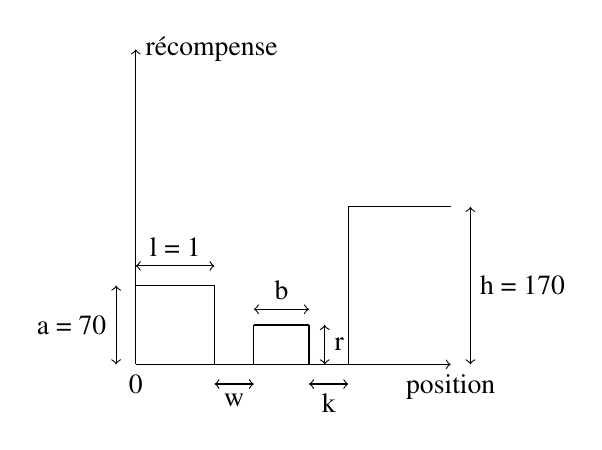
\begin{tikzpicture}
		% axe abscisse
		\draw[->] (1, 1) node[below] {0} -- (5, 1) node[below] {position};

		% axe ordonné
		\draw[->] (1, 1) -- (1, 5) node[right] {récompense};

		% premier palier
		\draw (1, 2) -- (2, 2);
		\draw (2, 1) -- (2, 2);

		% deuxieme palier
		\draw (2.5, 1) -- (2.5, 1.5);
		\draw (2.5, 1.5) -- (3.2, 1.5);
        \draw (3.2, 1.5) -- (3.2, 1);
        
        % troisieme palier
        \draw (3.7, 1) -- (3.7, 3.0);
        \draw (3.7, 3.0) -- (5.0, 3.0);

		% double fleche b
        \draw[<->] (2.5, 1.7) -- (3.2, 1.7) node[pos=.5, above] {b};
        
		% double fleche a
		\draw[<->] (0.75, 1) -- (0.75, 2) node[pos=.5, left] {a = 70};

		% double fleche r
        \draw[<->] (3.4, 1.0) -- (3.4, 1.5) node[pos=.5, right] {r};
        
		% double fleche l
		\draw[<->] (1, 2.25) -- (2, 2.25) node[pos=.5, above] {l = 1};

		% double fleche w
		\draw[<->] (2, 0.75) -- (2.5, 0.75) node[pos=.5, below] {w};
		
        % double fleche k
        \draw[<->] (3.2, 0.75) -- (3.7, 0.75) node[pos=.5, below] {k};
		% double fleche h
		\draw[<->] (5.25, 1) -- (5.25, 3) node[pos=.5, right] {h = 170};

		\end{tikzpicture}
		\caption{Illustration du second problème, les valeurs que nous avons prises sont les suivantes: w = k = 0.5, r = 30, b = 0.7.} \label{fig:probleme2}
	\end{figure}

Avant de débuter sur les explications de nos algorithmes, nous avons jugé important d'expliquer notre choix pour la distribution des valeurs des actions.
Pour rappel, la valeur d'une action $\in [0, 1]$. À partir de cela, 2 choix s'offre à nous afin de générer cette valeur aléatoirement; utiliser un générateur suivant la loi uniforme (figure \ref{fig:uniforme}), ou bien la loi normale (figure \ref{fig:normale}). 

Notre choix s'est finalement porté vers la loi normale, car nous avons jugé son comportement plus réaliste par rapport à notre problème. 

En effet, si nous prenons l'exemple d'un humain qui marche, nos pas ont approximativement la même valeur, autrement dit, nous avons plus de chance de faire un pas proche d'une certaine moyenne que d'enjamber quelque chose ou bien de faire des "micros" pas. C'est donc pour ce souci de réalisme que nous avons préféré la loi normale.



\begin{figure}[H]
\centering
  \begin{subfigure}{.4\textwidth}
    \centering
    	\includegraphics[width=.4\linewidth]{uniforme.png}
      \caption{loi uniforme}
  \label{fig:uniforme}
  \end{subfigure}
  \begin{subfigure}{.4\textwidth}
    \centering
        \includegraphics[width=.4\linewidth]{gaussien.png}
      \caption{loi normale}
  \label{fig:normale}
  \end{subfigure}
\caption{Exemple de distribution de valeurs}
\end{figure}


	\subsection{Première approche, modification du MCTS discret} \label{modifDiscret}

		Étant donné que nous avions passé quelque temps sur le MCTS discret, nous avons essayé de ré-utiliser ce dernier.

		Cependant, nous avons donc été confrontés à une première problématique : "Comment faire fonctionner un problème ayant des variables continues dans un algorithme fait pour des problèmes discrets ?" \\

		Et la réponse est simple, nous avons tout bonnement créé une entité permettant de faire la jonction entre le problème continu et notre MCTS discret qui, en programmation logicielle, correspond à un design pattern $Adapter$.\\

		Ci-dessous un diagramme de séquence simplifié (figure ~\ref{fig:actionsPossibles}), pour mieux comprendre, ce que donne ce système lorsque le MCTS va demander à un problème ses actions possibles.
		\begin{figure}[H]
			\centering
			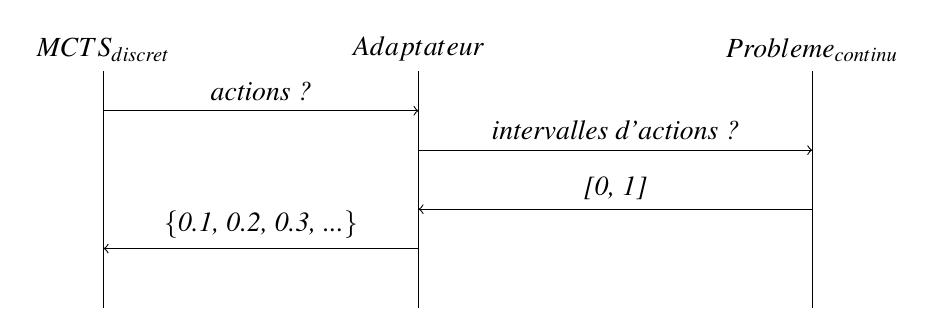
\begin{tikzpicture}
				% axe MCTS discret
				\draw (1, 2) -- (1, 5) node[above] {$MCTS_{discret}$};

				% axe adaptateur
				\draw (5, 2) -- (5, 5) node[above] {$Adaptateur$};

				% axe simulateur
				\draw (10, 2) -- (10, 5) node[above] {$Probleme_{continu}$};

				% segment actions ?
				\draw[->] (1, 4.5) -- (5, 4.5) node[pos=.5, above] { \textit{actions ?} };

				% segment intervalle d'actions ?
				\draw[->] (5, 4) -- (10, 4) node[pos=.5, above] { \textit{intervalles d'actions ?} };

				% segment réponse intervalle probleme->adaptateur
				\draw[->] (10, 3.25) -- (5, 3.25) node[pos=.5, above] { \textit{[0, 1]} };

				% segment réponse intervalle adaptateur->mcts
				\draw[->] (5, 2.75) -- (1, 2.75) node[pos=.5, above] { \textit{\{0.1, 0.2, 0.3, ...\}} };
			\end{tikzpicture}
			\caption{Obtenir les actions possibles d'un problème continu dans le MCTS discret} \label{fig:actionsPossibles}
		\end{figure}

À la différence des 2 prochaines variantes, cet algorithme ne nous permet pas de gérer les bruits parasites.
		
        Nous verrons dans la partie \ref{exp} que cette modification du MCTS discret est quasiment efficace que le progressive widening sans bruitage néanmoins, pour obtenir des résultats convaincants, nous devons modifier à la main certains paramètres, chose que fait dynamiquement le progressive widening.
        
	\subsection{Progressive widening} \label{pw}

		\subsubsection{Principe} \label{pw:principe}

		Contrairement à la version précédente, cette amélioration permet de résoudre des problèmes dont le nombre d'actions est très grand voire infini sans utiliser d'adaptateurs ou autres artifices.

		De plus, cet algorithme garde à peu près la même structure que l'algorithme générique MCTS (algorithme \ref{alg:mcts}), la principale différence est que les étapes $selection(n)$ et $simulation(n)$ sont regroupées en une seule étape, voir algorithme \ref{alg:mctspw}.
        Ces deux étapes sont maintenant réalisées par l'algorithme progressive widening, algorithme \ref{alg:spw} 

		Étant donné le fait que nous avons, pour tout nœud $n$, un nombre extrêmement grand d'actions possibles, cet algorithme va donc à chaque itération ajouter (ou non) à la liste des actions possibles d'un nœud courant, une ou plusieurs action(s) supplémentaire(s) puis créera au fur et à mesure un nouveau nœud pour chaque actions non développées.

		Afin de savoir si l'algorithme doit ajouter une ou plusieurs action(s), celui-ci va se baser sur la formule $Ct^\alpha$ avec $t$ le nombre de simulation et $C$ une constante d'exploration. Cette formule indiquera à l'algorithme s'il doit rajouter des actions possibles à sa liste d'actions ou non. Pour cela, le facteur d’accroissement de cette liste est donné par la variable $\alpha$ qui est comprise dans l'intervalle $]0, 1[$. 
        
        D'après la figure \ref{fig:variationsXPuissanceAlpha}, plus cette valeur sera proche de 0, moins l'algorithme créera de nouvelles actions possibles et donc favorisera la simulation des actions déjà existantes, on dira que l'algorithme favorise l'exploitation, tandis que plus $\alpha$ sera proche de $1$, plus celui-ci aura tendance à créer de nouvelles actions, on dira que l'algorithme favorise l'exploration, mais en contrepartie, il délaissera la simulation des actions déjà existantes. Dans le cas où $\alpha = 0.5$, l'algorithme aura tendance à ajouter des nouvelles actions vers le début et à diminuer cet ajout au fur et à mesure du temps. Il est donc intéressant de prendre un $\alpha$ proche de $0.5$ pour trouver un bon équilibre entre l'ajout de nouvelles actions possibles et la simulation des actions déjà existantes.

		\begin{figure}[H]
			\centering
                    \begin{tikzpicture}
                            \draw[->] (0,0) -- (5,0) node[anchor=north west] {x};
							\draw[->] (0,0) -- (0,5) node[anchor=south east] {$x^\alpha$};
                            
                            \draw[scale=1,domain=0:5,smooth,variable=\x,blue] plot({\x}, {\x^0});
                            \draw[scale=1,domain=0:5,smooth,variable=\x,red]  plot ({\x},{\x^1});
                            \draw[scale=1,domain=0:5,smooth,variable=\x,green]  plot ({\x},{\x^0.5});
                            
                            \draw[blue](6,5) -- (6.5,5);
                            \draw(7,5)node[]{$x^0$};
                            \draw[red](6,4.5) -- (6.5,4.5);
                            \draw(7,4.5)node[]{$x^1$};
                            \draw[green](6,4) -- (6.5,4);
                            \draw(7,4)node[]{$x^{0.5}$};
                    \end{tikzpicture}
			\caption{Variations de $x^\alpha$} \label{fig:variationsXPuissanceAlpha}
		\end{figure}

		Ce principe nous permet donc de développer de manière efficace les nœuds les plus visités, donc les nœuds plus intéressants.
        
       Comme annoncé en introduction, cet algorithme permet de gérer également un bruit parasite, cette action peut s'effectuer à la ligne \ref{pw:bruitage} de l'algorithme \ref{alg:spw}. Donc à chaque action choisit par l'algorithme, un bruit peut est ajouté. 
       
       Dans la partie \ref{exp}, nous avons effectué des tests en bruitant l'action choisi afin de comparer ces performances avec le double progressive widening \ref{dpw} puis nous avons ré-effectuer ces tests sans bruiter les actions.
		\begin{algorithm}[H]
			\caption{Progressive widening (PW) appliqué à un État $s$ avec la constante d'exploration $C > 0$ et $\alpha \in ]0, 1[$.}
			\label{alg:spw}
				\begin{algorithmic}[1]
					\Function{PW}{État $s$}
						\State $nbSimulation(s) \gets nbSimulation(s) + 1$ 
						\State $t \gets nbSimulation(s)$
						\State $k \gets \lceil{C \times t^{\alpha}}\rceil$
						\State \textit{// On va parcourir les actions possibles entre 0 et k}
						\For{$i \in [0 ,k]$}
							\State \textit{/* On récupère la récompense de s plus la récompense si on applique $action_{i}$ à $s$ */}
							\State $recompense \gets recompense(s) + recompense(s, action_{i})$
							\State \textit{// On récupère le nombre de simulation où $action_{i}$ a été appliqué à $s$}
							\State $nb \gets nbSimulation(s, action_{i})$
							\If{$nb = 0$}
								\State \textit{/* Si $action_{i}$ fournit un État jamais exploré, alors on retourne ce dernier */}
								\State \textbf{return} $(s, action_{i})$
							\Else
								\State \textit{// Sinon on calcul le score correspondant}
								\State $score(i) \gets \frac{recompense}{nb} + \textbf{$k_{ucb}$}\sqrt{\log(t)/(nb + 1)}$							
							\EndIf
						\EndFor
						\State \textit{// La boucle for est terminée, on recupère l'indice ayant le score maximal}
						\State $i_{max} \gets indiceMaximisant(score)$
						\State \textbf{return} $(s, action_{i_{max}})$ \textit{// bruitage possible ici} \label{pw:bruitage}
					\EndFunction
				\end{algorithmic}
		\end{algorithm}

		\begin{algorithm}[H]
			\caption{MCTS avec le progressive widening}
			\label{alg:mctspw}
				\begin{algorithmic}[1]
					\Function{MCTS}{État $s$}
						\While{$temps < tempsLimite $}\Comment{tant qu'il reste du temps}
							\While{$s$ n'est pas terminal}
								\State $s \gets PW(s)$ \Comment{On applique le progressive widening à $s$}
							\EndWhile
						\State $s \gets miseAjour(s)$
						\EndWhile
						\State \textit{/* Lorsque le temps est écoulé, on applique la stratégie robuste pour déterminer le meilleur prochain État */}
					\State \textbf{return} Robuste($s$)
					\EndFunction
				\end{algorithmic}
		\end{algorithm}
	\subsection{Double progressive widening} \label{dpw}

			Cette troisième variante, voir algorithme \ref{alg:dpw}, utilise la même logique que le progressive widening (section \ref{pw}).

	Cependant, au lieu d'ajouter, à chaque appel, un bruit à une action comme on peut le faire dans le progressive widening, cette méthode utilise la formule présente à la ligne \ref{choixEnfant} de l'algorithme \ref{alg:dpw}, or nous avons expliqué précédemment (figure \ref{fig:variationsXPuissanceAlpha}) comment se comporte une formule de ce type.
    
    Donc dans cet algorithme l'utilisation de cette formule nous permet de faire en sorte que, plus un nœud est simulé (donc s'il est souvent simulé, c'est que l'algorithme le trouve intéressant) plus il aura alors de chance d'être bruité. 
			
            De ce fait, en un seul appel, la fonction double progressive widening va produire à partir d'un état $s$ (potentiellement) 2 nœuds.

			Le premier nœud fils, noté $s'$, correspondra à la meilleure action $a$ appliqué à l'état $s$ (même principe que le progressive widening); puis le second nœud noté $s''$, un nœud fils de $s'$, correspondra à un bruit parasite appliqué à $s'$.
			
            Dans notre cas, le bruit est toujours additif, néanmoins l'algorithme est censé marcher peu importe si le bruit est additif ou soustractif.

			Donc, cet algorithme va nous permettre de gérer des situations dans lesquelles un événement tiers perturbe les résultats, type d’événement que l'on retrouve très souvent dans la vie de tous les jours. Par exemple, en hiver avec les plaques de verglas, il est possible de glisser légèrement sur l'une d'elles et donc de faire un pas plus grand que prévu, le bruit est ici la légère glissade.
            
            De plus, contrairement au progressive widening, cette variante développe de manière progressive le développement des actions à partir d'un nœud donné et aussi le développement des bruits parasites, d'où son nom "double élargissement progressif".

			\begin{algorithm}[H]
				\centering
				\caption{Double progressive widening (PW) appliqué à un État $s$ avec la constante d'exploration $C > 0$ et $\alpha \in ]0, 1[$.}
				\label{alg:dpw}
					\begin{algorithmic}[1]
						\Function{DPW}{État $s$}
							\State $nbSimulation(s) \gets nbSimulation(s) + 1$ 
							\State $t \gets nbSimulation(s)$
							\State $k \gets \lceil{C \times t^{\alpha}}\rceil$
							\State \textit{// On va parcourir les actions possibles entre 0 et k}
							\For{$i \in [0 ,k]$}
								\State \textit{/* On récupère la récompense de s plus la récompense si on applique $action_{i}$ à $s$ */}
								\State $recompense \gets recompense(s) + recompense(s, action_{i})$
								\State \textit{// On récupère le nombre de simulation où $action_{i}$ a été appliqué à $s$}
								\State $nb \gets nbSimulation(s, action_{i})$
								\If{$nb = 0$}
									\State \textit{// Si $action_{i}$ renvoit un état jamais exploré, alors on retourne cet état}
									\State \textbf{return} $(s, action_{i})$
								\Else
									\State \textit{// Sinon on calcul le score correspondant}
									\State $score(i) \gets \frac{recompense}{nb} + \textbf{$k_{ucb}$}\sqrt{\log(t)/(nb + 1)}$							
								\EndIf
							\EndFor
							\State \textit{// La boucle for est terminée, on recupère l'indice ayant le score maximal}
							\State $i_{max} \gets indiceMaximisant(score)$
							\State $s' \gets (s, action_{i_{max}})$ \Comment{On récupère le meilleur enfant dans s'}
							\State $nb \gets nbSimulation(s')$
							\State $nbEnfant \gets nbEnfant(s')$
							\State $k' \gets \lceil{C \times nb^{\alpha}}\rceil$ \label{choixEnfant}
							\If{$k' > nbEnfant$}
								\State $s'' \gets bruitage(s')$ \Comment{On applique un bruit à s'}
								\If{$s'' \notin enfants(s')$}
									\State $enfants(s') \gets enfants(s') \cup s''$ \Comment{On ajoute s'' comme enfant de s'}
									\State \textbf{return} $s''$ \Comment{On retourne l'enfant bruité}
								\Else
									\State \textbf{return} $s''$ \Comment{On retourne l'enfant bruité}
								\EndIf
							\Else
								\State \textit{// Sinon on retourne un enfant tiré aléatoirement dans s'}
								\State \textbf{return} $enfantAleatoire(s')$
							\EndIf
						\EndFunction
					\end{algorithmic}
			\end{algorithm}
			
			L'algorithme \ref{alg:mctsdpw} correspond à l'algorithme MCTS où la stratégie double progressive widening est appliquée. 
			\begin{algorithm}[H]
			\centering
			\caption{MCTS avec le double progressive widening}
			\label{alg:mctsdpw}
				\begin{algorithmic}[1]
					\Function{MCTS}{État $s$}
						\While{$temps < tempsLimite $}\Comment{tant qu'il reste du temps}
							\While{$s$ n'est pas terminal}
								\State $s \gets DPW(s)$ \Comment{On applique le double progressive widening à $s$}
							\EndWhile
						\State $s \gets miseAjour(s)$
						\EndWhile
						\State \textit{/* Lorsque le temps est écoulé, on applique la stratégie robuste pour déterminer le meilleur prochain État */}
					\State \textbf{return} Robuste($s$)
					\EndFunction
				\end{algorithmic}
		\end{algorithm}
\subsection{Expérimentations} \label{exp}
	
    Dans cette partie, nous allons comparer les différents algorithmes décrit dans la partie \ref{continu} au problème (partie \ref{probleme}, figure \ref{fig:probleme1}), puis pour valider les performances de nos algorithmes, nous testerons uniquement le progressive widening ainsi que le double progressive widening sur le problème 2 (partie \ref{probleme}, figure \ref{fig:probleme2}) jugé plus complexe dans la partie \ref{exp:resMonde2}.\\
    
    Dans la partie \ref{exp:MCTSvsPW}, nous allons comparer les performances entre l'algorithme MCTS décrit à la partie \ref{modifDiscret} et le progressive widening sans bruitage (partie \ref{pw}).

Puis nous comparerons dans la partie \ref{exp:PWvsDPW}, les performances du double progressive widening (partie \ref{dpw}) et du progressive widening (partie \ref{pw}) avec bruitage. 
	
    Dans tous les tests, la formule de sélection finale est la stratégie robuste (voir partie \ref{selectionFinale}) et la valeur de $R$ du bruit a été fixé à $0.05$. \\
    
    Ces tests ont été effectués sur un ordinateur avec un processeur i7 avec $16$ Go de RAM.

	\subsubsection{Expérimentations sur le MCTS discret et le progressive widening sans bruitage} \label{exp:MCTSvsPW}  
    
    Notre première expérimentation va consister tout simplement à exécuter $500$ fois ces 2 algorithmes avec la même valeur de temps, soit $10$ms, sur le problème 1 (figure \ref{fig:probleme1}). D'après notre compréhension de ces 2 algorithmes, nous devrions obtenir des résultats quasiment identiques.
    
    Étant donné que ces 2 algorithmes ne sont pas strictement similaires, nous sommes obligés de faire varier une variable afin d'essayer de rendre leurs 2 comportements plus proches :
\begin{itemize}
\item Pour l'algorithme MCTS, la variable à faire varier est la valeur de l'échantillonnage. En effet, cette valeur correspond au nombre d'actions maximales que nous accordons à un nœud donné, par exemple si nous fixons cette valeur à 10, cela signifie donc qu'un nœud pourra avoir au maximum 10 actions différentes, i.e 10 nœuds fils différents.
\item Pour le progressive widening, la variable à faire fluctuer est la constante d'exploration $C$ car c'est elle qui va indiquer à l'algorithme combien d'échantillonnage il s’autorise à prendre, voir notre explication dans la partie \ref{pw}.
\end{itemize}
    
    Suite à ces 500 simulations, nous obtenons les figures \ref{fig:adapterNonBruite} et \ref{fig:pwNonBruite}, et il est intéressant de remarquer que la moyenne des récompenses augmente légèrement voir stagne jusqu'à un seuil (différents pour les deux algorithmes) puis fait chuter de manière brutale la moyenne des récompenses, la faisant ainsi passer pour l'algorithme MCTS de 152 à 117, et de 170 à 115 pour le progressive widening. 
    
    Ce phénomène vient du fait que les algorithmes développent beaucoup de nouveaux nœuds, et passent donc peu de temps à les exploiter. On a donc trop favorisé l'exploration de l'arbre au dépit de l'exploitation. Donc dans ce cas, favoriser l'exploration entraîne la détérioration des résultats.
    
    De plus, notre formule de sélection finale est la stratégie robuste, or cette stratégie est censée nous retourner le nœud enfant possédant le plus de simulation, donc si nos algorithmes ne font qu'explorer l'arbre, nous pouvons supposer que la valeur de simulation de la plupart des nœuds créés est proche de 1. Donc il est tout à fait possible que cette stratégie nous retourne dans ce cas un nœud ayant une très mauvaise valeur de récompense (resp. très bonne).
    
    Nous pouvons également remarquer grâce à la table  \ref{tabular:intervalesEchantillonsPWNonBruite} que le progressive widening développe nettement moins de nœud par rapport à l'algorithme MCTS. Ce gain lui permet d'être en plus de performant, économe en ressources.
    
    \begin{figure}[H]
		\centering
		\includegraphics[width=\textwidth]{AdapterNonBruite.pdf}
		\caption{Variations de l'adaptateur MCTS discret en fonction du nombre d’expérimentations, $ErreurStandard_{MCTSdiscret} = [0.32 ; 0.06 ; 0.66 ; 1.72]$}
		 \label{fig:adapterNonBruite}
	\end{figure}
    
    \begin{figure}[H]
		\centering
		\includegraphics[width=\textwidth]{PWNonBruite.pdf}
		\caption{Variations de PW non bruité en fonction de C, $ErreurStandard_{PW} = [0.67 ; 0.66; 0.67 ; 0.63 ; 0.52 ; 0.20 ; 0.06 ; 1.72 ; 1.66 ; 1.72 ; 1.71]$}
		 \label{fig:pwNonBruite}
	\end{figure}
    
    \begin{table}[H]
    		\centering
    		\begin{tabular}{ | *{12}{c|}}
    				\hline
                    C											  & 1 & 2 & 3 & 5 & 8 & 10 & 21 & 34 & 55 & 89 & 144   \\ \hline
                    Échantillonnage min		& 31 & 59 & 71 & 95 &  117 & 151 & 195 & 209 & 149 & 133 & 105   \\ \hline
                    Échantillonnage max	   & 41 & 61 & 76 & 100 & 126 & 160 & 207 & 255 & 259 & 263 & 259   \\ \hline
    		\end{tabular}
			\caption{Intervalles des échantillons obtenus en faisant variant C pour le PW non bruité}\label{tabular:intervalesEchantillonsPWNonBruite}
    \end{table}

	\subsubsection{Expérimentations sur le progressive widening avec bruitage et le double progressive widening} \label{exp:PWvsDPW}
    
    Cette seconde expérimentation vise donc à comparer deux algorithmes permettant la gestion de bruits parasites. Il est donc inutile ici de les comparer à notre précédent algorithme MCTS et, comme dit dans la partie précédente (\ref{exp:MCTSvsPW}), le progressive widening est bien plus efficace.
    
    Lorsque nous faisons varier la constante d'exploration $C$, les résultats obtenus (Figure \ref{fig:VariationDeC_PWvsDPW}) montre globalement que l'algorithme double progressive widening a toujours une valeur moyenne de récompense supérieure à celle de l'algorithme progressive widening. 
    
    Il est aussi intéressant de remarquer que, comme dans la partie \ref{exp:MCTSvsPW}, à partir de la valeur $C=21$ les performances de l'algorithme double progressive widening chute, passant ainsi de 161 à 120 de moyenne. Alors que l'algorithme progressive widening reste stable sur ce domaine. 
    
    De plus, nous pouvons remarquer que les écart-types des récompenses moyennes sont beaucoup plus faibles (pour $C <= 21$) pour le double progressive widening par rapport à ceux du progressive widening. 
    Cela indique une plus grande précision dans les résultats. 
    
    Néanmoins, lorsque $C>21$, les valeurs d'écart-types du double progressive widening deviennent plus importantes, nous pouvons expliquer cela par le fait que l'algorithme tombe plus souvent dans le piège du problème. 
    
    En effet, pour rappel si notre algorithme tombe dans le piège sa récompense sera de 70; alors que s'il arrive à accéder à la plate-forme finale sa récompense sera de 170. De ce fait si nos résultats finaux alternent énormément entre 70 et 170, notre moyenne va tendre vers 120 et notre écart-type sera également grand.
    
    Donc le comportement observé pour le double progressive widening à partir de $C>21$ est explicable.
    
    
    \begin{figure}[H]
		\centering
		\includegraphics[width=\textwidth]{VariationDeC_PWvsDPW.pdf}
		\caption{Variations des moyennes de récompenses en fonction de $C$ pour PW et DPW avec $\alpha = 0.4$ et le $temps = 10$, $ErreurStandard_{PWbruité} = [1.71 ; 1.74 ; 1.66 ; 1.67 ; 1.69 ; 1.73 ; 1.69 ; 1.70 ; 1.64 ; 1.71 ; 1.66]$, $ErreurStandard_{DPW} = [0.80 ; 0.79 ; 0.67 ; 0.77 ; 0.60 ; 0.84 ; 1.24 ; 1.72 ; 1.69 ; 1.71 ; 1.74]$}
		 \label{fig:VariationDeC_PWvsDPW}
	\end{figure}
    
    Posons $C=8$ et faisons maintenant varier la variable $\alpha$, nous pouvons remarquer sur la figure \ref{fig:VariationDAlpha_PWvsDPW} que le même phénomène qu'énoncé précédemment se produit, c'est-à-dire qu'à partir d'une certaine valeur (liée à $\alpha$), l’efficacité du double progressive widening va grandement chuter tandis que le progressive widening va stagner au niveau des récompenses mais globalement,
    les performances du double progressive widening sont toujours supérieures à celle du progressive widening simple.
    
    Expliquons maintenant pourquoi la valeur d'$\alpha$ peut causer des problèmes de performances. 
    Pour rappel, dans le double progressive widening nous utilisons à 2 reprises la variable $\alpha$ (voir algorithme \ref{alg:dpw}), la première occurrence d'$alpha$ est : $C \times t^\alpha$ avec $t$ le nombre de simulation d'un nœud $n$.
    
    Donc si $alpha$ est égal à $0$ (cas qui n'est pas admis par l'algorithme, mais intéressant à observer), alors le nœud $n$ pourra avoir uniquement $C$ actions possibles, car peu importe la valeur de $t$, celle-ci à la puissance $0$ donnera tout le temps $1$. De même, le double progressive widening ne pourra ajouter qu’au maximum $C$ bruits à chacun de ces nœuds enfants. Alors, comment expliquer que l'algorithme arrive tout de même à avoir une récompense respectable ? 
    La réponse est simple, nos valeurs de pas suivent la loi normale.
    
    Intéressons-nous maintenant au cas où $\alpha = 1$ (cas également non admis), alors l'algorithme à chaque nouvel appel pour un noeud $n$ va lui indiquer qu'il a de nouvelles actions disponibles, car la formule étant : $C \times t^\alpha$ avec $t$ le nombre de simulation d'un nœud, si $\alpha=1$ on se retrouve alors avec $C \times t$ et sachant que $t$ croît de manière linéaire, on ajoute donc $C$ actions possibles à chaque appel. Et donc, notre algorithme passe beaucoup de temps à explorer l'arbre au lieu de l'exploiter.
    
    D'où l'important pour la suite, de choisir une valeur intermédiaire de $\alpha$, proche de $0.5$.
    
    \begin{figure}[H]
		\centering
		\includegraphics[width=\textwidth]{VariationDAlpha_PWvsDPW.pdf}
		\caption{Variations des moyennes de récompenses en fonction d'alpha pour PW et DPW avec $C = 8$ et le $temps = 10$, $ErreurStandard_{PWbruité} = [1.66 ; 0 ; 1.69 ; 1.67 ; 1.68 ; 1.71 ; 1.66 ; 1.71 ; 1.70 ; 1.70 ; 1.72]$, $ErreurStandard_{DPW} = [0.84 ; 0.82 ; 0.70 ; 0.69 ; 0.57 ; 0.78 ; 1.29 ; 1.67 ; 1.69 ; 1.72 ; 1.72]$}
		 \label{fig:VariationDAlpha_PWvsDPW}
	\end{figure}
    
    
    Maintenant que nous connaissons les conséquences liées aux variables $C$ et $\alpha$, faisons varier le temps de réflexion de l'ordinateur en fixant cette fois-ci $C$ à $8$ et $\alpha$ à $0.6$.
    Nous remarquons grâce à la figure \ref{fig:VariationDuTemps_PWvsDPW}, que si le temps de réflexion n'est pas assez grand, le double progressive widening aura les mêmes résultats en moyenne que son homologue progressive widening mais plus le temps croît plus le double progressive widening aura de meilleurs récompenses en moyenne que le progressive widening mais, une fois la valeur de temps $T=8$ms les moyennes des deux algorithmes commencent à stagner. 
    
    Donc la figure \ref{fig:VariationDuTemps_PWvsDPW} nous permet de savoir qu'il n'est pas utile de laisser réfléchir trop longtemps ces deux algorithmes.
    
    \begin{figure}[H]
		\centering
		\includegraphics[width=\textwidth]{VariationDuTemps_PWvsDPW.pdf}
		\caption{Variations des moyennes de récompenses en fonction du temps (en ms) pour PW et DPW avec $C = 8$ et $\alpha = 0.6$, , $ErreurStandard_{PWbruité} = [1.71 ; 1.68 ; 1.70 ; 1.74 ; 1.69 ; 1.78 ; 1.73 ; 1.71 ; 1.69 ; 1.67 ; 1.71]$, $ErreurStandard_{DPW} = [1.68 ; 1.74 ; 1.47 ; 1.42 ; 1.32 ; 1.19 ; 1.19 ; 0.98 ; 1.06 ; 1.08 ; 0.76]$}
		 \label{fig:VariationDuTemps_PWvsDPW}
	\end{figure}

    Suite à tous ces tests, nous en avons déduit qu'une bonne combinaison de valeurs était $C = 8$, $\alpha = 0.6$ et $T = 34$ms. 
    
    La figure \ref{fig:comparatif_resultat_final_en_pourcent} montre la répartition des récompenses en pourcentage.
    
    Nous pouvons clairement observer que le double progressive widening est bien meilleur que le progressive widening. En effet, celui-ci atteint à plus de 90\% la récompense optimale contre seulement 15\% pour le simple progressive widening. 
    
    Malgré les 10\% de score à 70 i.e le double progressive widening tombe 1 fois sur 10 dans le piège. Il est tout de même préférable de choisir cet algorithme dans le cas où nous avons un problème dans un monde continu où un bruit parasite se produit.
    
      \begin{figure}[H]
		\centering
		\includegraphics[width=\textwidth]{comparatif_resultat_final_en_pourcent.pdf}
		\caption{Pourcentage de score obtenu pour PW et DPW avec $C = 8$, $\alpha = 0.6$ et $T = 34$}
		 \label{fig:comparatif_resultat_final_en_pourcent}
	\end{figure}
    
    
    
    
    \subsubsection{Expérimentation sur le problème 2} \label{exp:resMonde2}
    
    Dans cette partie nous avons juste voulu vérifier si le problème (figure \ref{fig:probleme2}) contenant cette fois-ci 2 pièges était encore réalisable par les algorithmes progressive widening et double progressive widening. 
    
    Les résultats obtenus sur la figure \ref{fig:comparatif_resultat_final_en_pourcent_monde 2} confirme la supériorité du double progressive widening face au progressive widening dans un monde continu stochastique. En effet, dans ce problème la récompense optimale est de 270 et, comme nous pouvons l'observer, l'algorithme double progressive widening arrive à atteindre cette récompense plus de 95\% des fois, soit environ 20\% de plus que le progressive widening.
    
      \begin{figure}[H]
		\centering
		\includegraphics[width=\textwidth]{comparatif_resultat_final_en_pourcent_monde2.pdf}
		\caption{Pourcentage de score obtenu pour PW et DPW avec $C = 8$, $\alpha = 0.6$ et $temps = 34$}
		 \label{fig:comparatif_resultat_final_en_pourcent_monde 2}
	\end{figure}
    
    Donc même en modifiant le monde et en rajoutant une difficulté supplémentaire, l'algorithme double progressive widening arrive tout de même à obtenir la récompense maximale de manière plus fiable que son homologue progressive widening.
    

\subsection{Conclusion}

L'algorithme de décision \textbf{M}onte \textbf{C}arlo \textbf{T}ree \textbf{S}earch \cite{coulom01} est très facilement adaptable à toutes sortes de mondes, tantôt il peut être utilisé dans un monde discret (partie \ref{P4}) tantôt il peut être adapté à un monde continue (partie \ref{continu}).

Cependant, cette dernière adaptation se fait avec plus ou moins de réussite, en effet si nous voulons réutiliser le MCTS discret (partie \ref{modifDiscret}) nous devons manuellement indiquer combien de valeurs d'actions nous souhaitons échantillonner, puis ajuster ce paramètre par rapport aux précédents résultats, ceci est très fastidieux et peu dynamique.
	
    Or, le progressive widening (partie \ref{pw}) permet d'effectuer cet échantillonnage de façon dynamique, et est également plus performant que le MCTS discret (voir figures \ref{fig:adapterNonBruite} et \ref{fig:pwNonBruite}) sur notre premier problème.
    De plus, nous avons remarqué que lorsque le progressive widening ne gérait pas les bruits (figure \ref{fig:pwNonBruite}) sa moyenne de récompense tend vers $170$ pour $C <= 21$ soit la valeur optimale. 
    
    Donc, nous pouvons supposer que si nous avons un problème dans un monde continu où aucun bruit parasite risque de se produire alors l'utilisation du MCTS avec le progressive widening peut être une bonne initiative.
    
    
    Maintenant, si nous nous retrouvons dans une situation où le monde est continu et où des bruits aléatoires risquent de se produire alors nous pensons qu'il est préférable d'utiliser le double progressive widening, car ces performances sont globalement meilleures que celle du progressive widening bruité (figure \ref{fig:VariationDuTemps_PWvsDPW}).
    \\ \\
    Donc nous avons pu déterminer qu'il était possible de planifier des actions dans un monde continu en utilisant un algorithme tel que le \textbf{M}onte \textbf{C}arlo \textbf{T}ree \textbf{S}earch, néanmoins il serait intéressant de voir s'il est également possible de gérer la planification d'actions dans un monde continu \textbf{et} dynamique.




\newpage
\selectlanguage{french}
\bibliographystyle{alpha}
\bibliography{biblio.bib}

\end{document}